The output of the data-processing pipeline described in \sref{data} is the data
set $X$, which is split into three parts: $X_1$ is for the training stage, $X_2$
for the validation stage, and $X_3$ for the testing stage. In what follows, we
elaborate on the processes that are taking place during these three stages of
working with the model presented in \sref{model}.

\subsection{Training} \slab{training}
The model in \sref{model} has a large number of parameters that have to be
learned during training; they are primarily various weights and biases inside
the layers. For this purpose, $X_1$ is utilized. The training is undertaken via
backpropagation through time using stochastic gradient descent
\cite{goodfellow2016} whose objective is to minimize a certain loss function,
which we shall specify shortly. There are two aspects to be discussed first.

\begin{figure}[t]
  \centering
  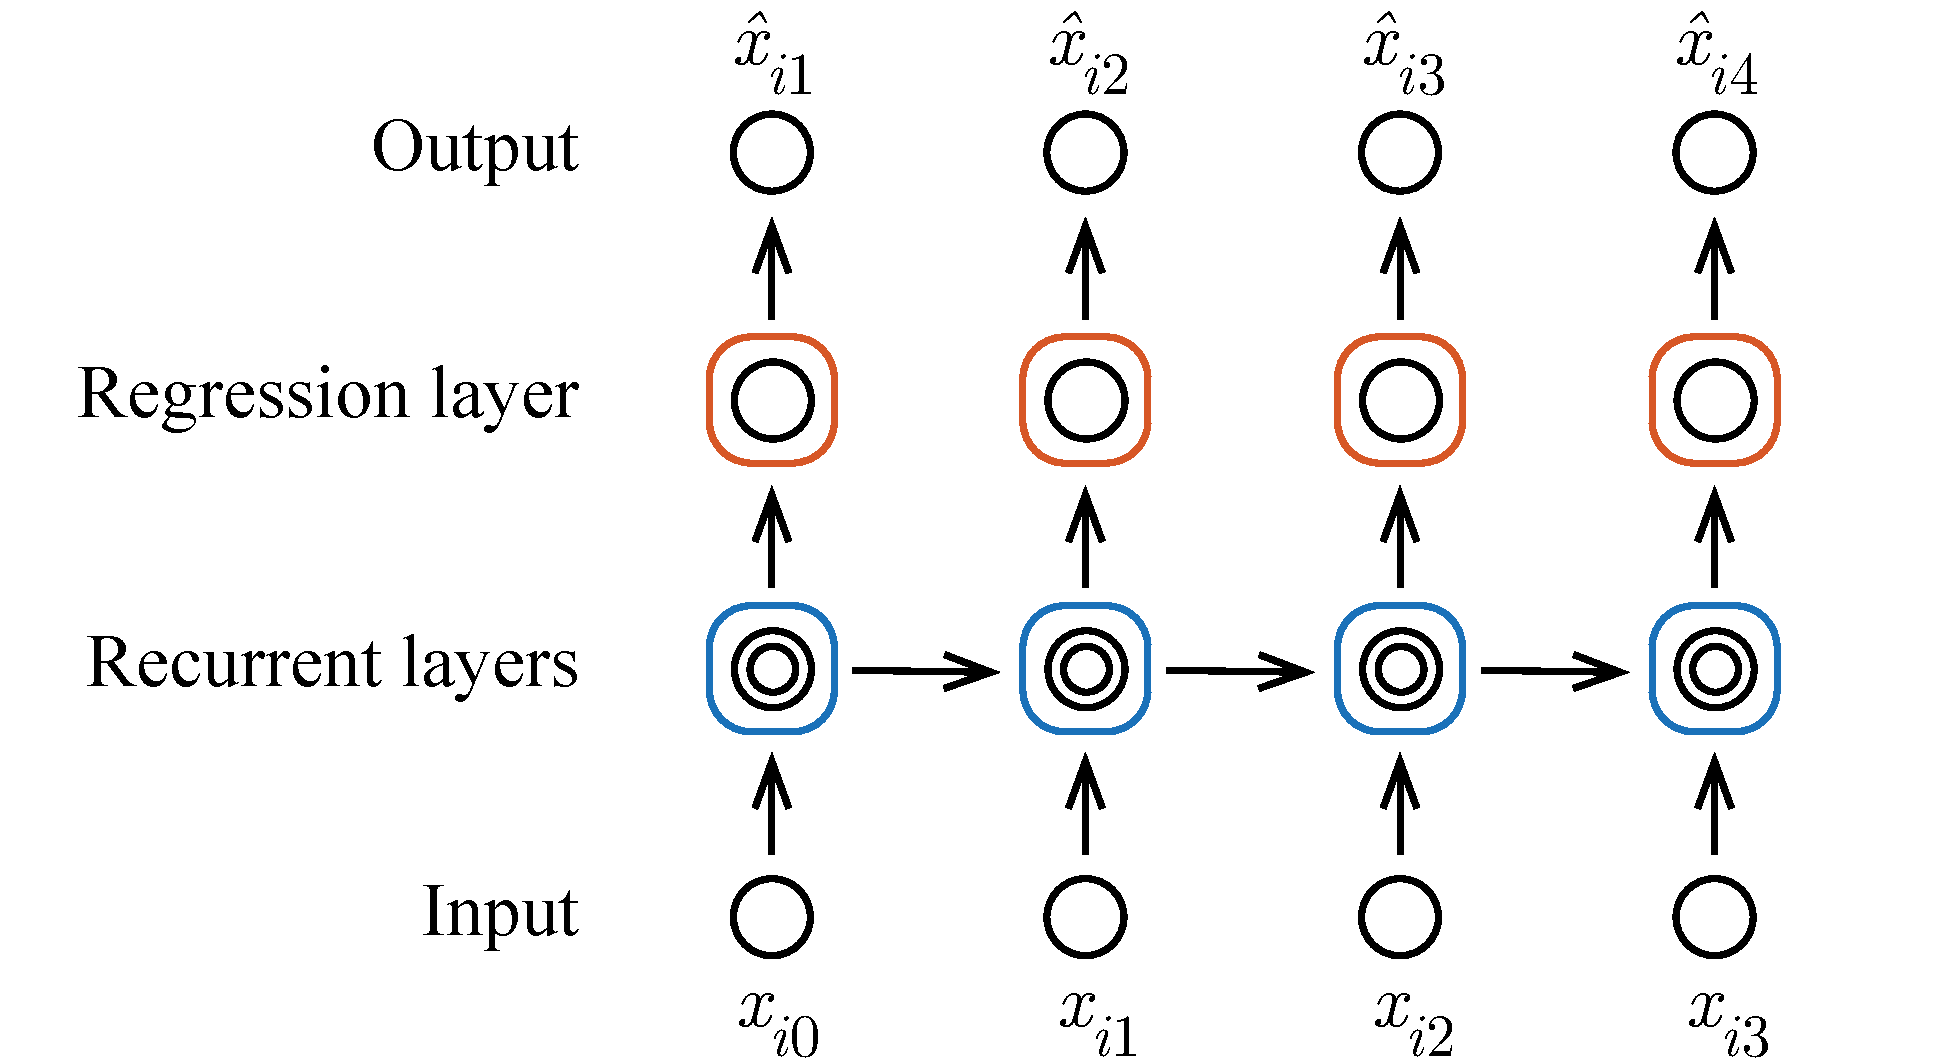
\includegraphics[width=1.0\columnwidth]{include/assets/figures/unroll.pdf}
  \vspace{-2.0em}
  \caption{Example of dynamic unrolling during the model's usage.}
  \vspace{-1.5em}
  \flab{unroll}
\end{figure}

The first concerns the way a single resource-usage trace is fed into the model.
To begin with, the internal memory is nullified before feeding a trace. Next,
note that a trace, as in \eref{trace}, has multiple data points ($l_i > 1$), and
that two traces are likely to have different lengths ($l_i \neq l_j$) since the
execution times of two tasks are likely to differ. With this in mind, all the
points of a trace are fed in one pass using a technique called dynamic
unrolling. An illustration for $l_i = 4$ is given in \fref{unroll}, in which the
representation in \fref{model} has been simplified even further and rotated
$90^\circ$ counterclockwise. It can be seen that the model has been replicated
as many times as there are data points in the trace. However, it is still the
same model, and all the replicas share the same parameters and internal memory.
It can also be seen in \fref{unroll} how information flows from one time step to
the next, which is what makes the model recurrent.

Now, it is not efficient to feed only one trace at a time due to the inevitable
overhead imposed by the computations involved. Therefore, these computations
should be performed in batches whenever possible. Since $l_i \neq l_j$ in
general, it is not possible to stack multiple arbitrary traces into a single
tensor directly. In order to circumvent this problem, we reside to bucketing.
Specifically, each read trace is put into one of many queues depending on its
length. When a queue, accumulating traces of length from some $l'$ to $l''$, has
collected the desired number of traces---denoted by $b$ and referred to as the
batch size---it pads traces shorter than $l'$ with zeros and emits a tensor of
size $b \times l'' \times d$ to be further consumed by the model.

The loss function that we minimize during training is the mean squared error
(\up{MSE}) \cite{hastie2009} of one-step predictions over the whole batch. The
correct prediction for the very last time step, which goes beyond the time
window of the traces in question, is assumed to be zero. For instance, in
\fref{unroll}, $\hat{x}_{i4}$ has no $x_{i4}$ to be compared with; $x_{i4}$ is
assumed to be zero.

\subsection{Validation} \slab{validation}
As it is the case with arguably all nontrivial machine-learning models, the one
presented in \sref{model} has a number of hyperparameters. Examples include the
number of cells $c$, number of units per cell $u$, and probability of dropout
$p$, which are introduced in \sref{recurrent}. Unlike (ordinary) parameters,
which are to be optimized during training (see \sref{training}), such
hyperparameters are to be set prior to training, and they are typically kept
unchanged thereafter. From the examples given, it is apparent that the impact of
hyperparameters is profound. Therefore, they should be carefully configured.

The validation set $X_2$ is used to assess the performance of the model trained
(using $X_1$ as usual) under different configurations of the model's
hyperparameters. As before, the error metric is the \up{MSE}, and it is highly
beneficial to perform these computations in batches. The trained model that has
the best performance on $X_2$ is then chosen as the final one.

Despite all the techniques employed to speed up training, it is still an
expensive operation. As a result, brute-force search in the space of
hyperparameters for the best configuration is impractical; a certain intelligent
strategy should be followed.

In our workflow, we use the Hyperband algorithm \cite{li2016}. Instead of
adaptively choosing new configurations to evaluate---which is the case with many
algorithms of this kind---it adaptively allocates resources to configurations
chosen at random, which has been shown to be a very efficient strategy. In
particular, the algorithm allows one for saving a lot of compute power, which
otherwise would be burnt in vain evaluating overtly inadequate configurations of
hyperparameters. In this context, \emph{resources} refers a user-defined measure
of how extensively a configuration is exercised. For instance, it can be the
amount of wall-clock time spent or the number of training steps taken; in our
experiments, we use the latter.

\subsection{Testing} \slab{testing}
After a trained model has been selected during the validation stage, the model
has to be assessed anew \cite{hastie2009}: one cannot aver that the error with
respect to $X_2$ is the generalization error of the model because the selection
was biased (we deliberately chose the one that performed the best on $X_2$).

In order to have an unbiased evaluation, the testing set $X_3$ is utilized. As
it is with training and validation, the \up{MSE} is considered as a quality
metric, and the bucketing mechanism is used (see \sref{training}). However,
unlike training and validation, the error is calculated in a more elaborate way
as follows.

Recall first that our objective is making long-range predictions of resource
usage (see \sref{problem}). Note also that, in \sref{training} and
\sref{validation}, we are only concerned with what happens one time step ahead.
The reason is that we would like to have as high of a throughput as possible
since the training and validation operations are to be performed many times.
Testing, however, is done only once, and it is during testing we make and assess
multiple-step-ahead predictions.

In order to compute long-rage predictions, we use refeeding: at time step $k$,
the predicted value $\hat{x}_{i,k + 1}$ is fed into the model as if it was the
actual resource usage $x_{i,k + 1}$ at step $k + 1$, which is not yet known at
step $k$. The process continues until all the desired $h$ future values are
estimated. It is natural to expect that the more accurate the one-step-ahead
prediction is, the more accurate the multiple-step-ahead one will be.

There is more to it. Consider how a trained model will be used in practice.
Potentially at each step $k$, one might want to predict the next $h$ values of
the resource usage of task $i$, that is, $\hat{x}_{i,k + 1}, \dots, \hat{x}_{i,k
+ h}$. Therefore, in order to test the model properly, we have to sweep over all
the time steps of the trace in question while making $h$ predictions at each
step. An important aspect to note here is that the state of the model's memory
should be saved before computing $\hat{x}_{i,k + 1}, \dots, \hat{x}_{i,k + h}$
at step $k$ and restored before feeding $x_{i,k + 1}$ in order to advance to
step $k + 1$. The memory becomes contaminated when one feeds predictions instead
of observations into the model.

It can be seen in the presentation above that testing is a rather elaborate
operation involving sequential computations.

At this point, the main aspects of our workflow have been discussed, and we move
on to the experimental results.
